\chapter{Preliminares}
La ciencia de datos es el campo que aplica técnicas analíticas avanzadas y principios científicos para extraer información valiosa de los datos. Su objetivo principal es la extracción, el análisis y la comunicación de información útil a partir de los datos. Combina la estadística, la informática y el pensamiento crítico para obtener conocimiento significativo y relevante. Para realizar un análisis de datos, es necesario tener conocimientos en matemáticas, estadística, programación, inteligencia artificial, aprendizaje automático y experiencia en diversas áreas de aplicación. En este caso, es indispensable incursionar en conocimientos de genómica y metagenómica.\\

En microbiología, un factor importante de estudio son las interacciones entre microorganismos en un ambiente natural, ya que la mayoría de estos estudios se realizan en laboratorios. Los avances tecnológicos han llevado al desarrollo de métodos de secuenciación de ADN. Una de las plataformas más utilizadas y conocidas en el campo de la metagenómica es Illumina. Con este tipo de herramientas, es posible analizar el ADN extraído directamente de una muestra, en lugar de trabajar únicamente con microorganismos cultivados individualmente.\\

La filogenética es el estudio de la evolución de la vida y las relaciones entre organismos y grupos de organismos. Este análisis se centra en temas como la diversidad, la evolución, la ecología y los genomas, ayudándonos a comprender cómo evolucionan los genes, los genomas y las especies. Una parte importante de este estudio es la identificación, clasificación y denominación de organismos biológicos, campo conocido como taxonomía. Carl Linnaeus, considerado el padre de la taxonomía, propuso siete niveles taxonómicos: Reino, Phylum, Clase, Orden, Familia, Género y Especie. Posteriormente, se añadió el Dominio como el octavo grupo taxonómico más amplio, dividido en Arqueas, Bacterias y Eukarya.\\

\begin{figure}[h]
\centering
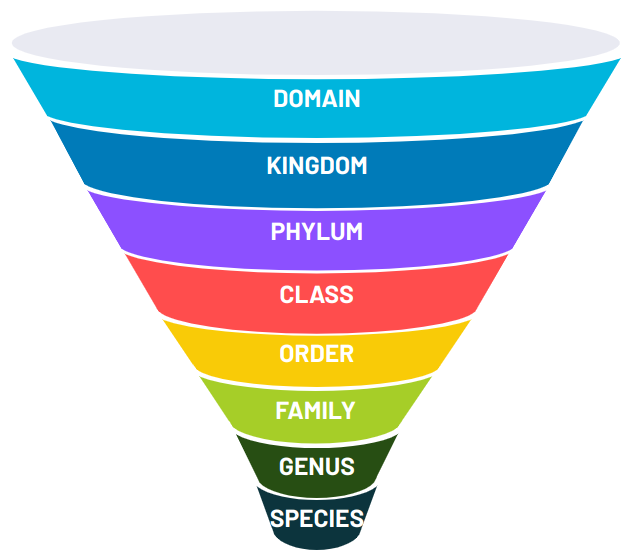
\includegraphics[scale=0.3]{Img/cap1/taxonomic.png}
\label{Fig 1.1}
\caption{Representación Jerárquica de los Niveles Taxonómicos para la Clasificación y Análisis de Datos Metagenómicos}
\end{figure}


Los niveles taxonómicos \ref{Fig 1.1} son categorías jerárquicas utilizadas para clasificar organismos, desde los grupos más generales hasta los más específicos. El Reino es el nivel más amplio y agrupa organismos según características fundamentales, como ser procariotas o eucariotas. Dentro de cada reino, los organismos se subdividen en Filos, que los organizan según estructuras o procesos biológicos compartidos. Estos se clasifican en Clases, que reúnen grupos más específicos de organismos. A su vez, las clases se dividen en Órdenes, que contienen familias relacionadas. Las Familias agrupan Géneros, que son conjuntos de especies estrechamente relacionadas. Finalmente, la Especie es el nivel más específico, que incluye organismos capaces de reproducirse entre sí y producir descendencia viable. Esta jerarquía es esencial para organizar la biodiversidad y estudiar las relaciones evolutivas entre los organismos.\\

\section{Metagenómica}
La metagenómica es el estudio integral del material genético recuperado directamente de muestras ambientales. Permite analizar el genoma colectivo (metagenoma) de todos los microorganismos presentes en un ambiente determinado, sin necesidad de cultivarlos individualmente. Este campo se centra en comprender la diversidad microbiana, las estructuras poblacionales, las capacidades funcionales y las interacciones de las comunidades microbianas con su entorno. Se aplica comúnmente en el estudio de ecosistemas como el suelo, el agua, la microbiota humana y otros hábitats microbianos complejos. La metagenómica utiliza tecnologías avanzadas de secuenciación, como la secuenciación de nueva generación, para desentrañar la diversidad genética y funcional de estas comunidades (Zhang, 2021).\\

Existen dos enfoques para la secuenciación de microorganismos: “Amplicón 16S rRNA” y “Shotgun”. La secuenciación por amplicón 16S fue el primer método de secuenciación metagenómica altamente aceptado. Tiene muchas ventajas: el gen 16S está presente en todas las bacterias y arqueas, contiene las regiones necesarias para un buen análisis de PCR (Polymerase Chain Reaction - Reacción en Cadena de la Polimerasa) altamente conservadas, existen conjuntos de primers altamente estudiados para amplificar la mayoría de los organismos, ya se encuentran disponibles bases de datos públicas y bien seleccionadas que permiten una buena comparación, y la secuenciación por 16S es relativamente barata y simple. Sin embargo, posee algunas desventajas: el gen 16S no está presente en los hongos, por lo que este método no es adecuado cuando se desea trabajar con hongos. Además, existe la posibilidad de que se incremente el error de sesgo si no se elige el conjunto de primers adecuado para el organismo a analizar.\\

Para realizar una secuenciación por 16S, es necesario seguir una serie de pasos para la preparación de la muestra biológica y la extracción del ADN: colecta de la muestra, extracción del ADN y preparación de la librería. Para la colecta de las muestras, se deben tener en cuenta las necesidades del experimento y los resultados esperados, estimar el número de muestras necesarias y considerar el método de almacenamiento; todo esto para garantizar la calidad de los datos. Existen varios métodos y herramientas para realizar la extracción del ADN. Es necesario preparar bibliotecas de datos genómicos para la comparación de las secuencias. Posteriormente, se continúa con la secuenciación de las muestras, para lo cual existen varias herramientas, siendo una de las más usadas Ilumina, que ofrece una mayor cobertura a menor costo. Finalmente, se realiza un control de calidad, cuyo principal objetivo es mejorar la precisión del análisis y prevenir la sobreestimación de los datos. El control de calidad puede incluir: la detección y eliminación de quimeras artificiales, el filtrado de secuencias de baja calidad y de reads muy cortos, así como la eliminación de ruido.\\

Una vez obtenidas las secuencias, es necesario identificar el grupo taxonómico correspondiente para cada secuencia. Para esto, se conocen dos enfoques principales: uno basado en filotipos, que agrupa las secuencias directamente en función de su similitud con los filotipos, y otro basado en OTUs (Unidades Taxonómicas Operacionales), que agrupa las secuencias según la similitud entre OTUs. El método de agrupación por OTUs supera al basado en filotipos, pero también presenta ciertas limitaciones, ya que es relativamente costoso computacionalmente y requiere mucha memoria. Un OTU se define dentro del mismo clúster por un porcentaje de similitud, siendo el 97\% un porcentaje común a nivel de especie. Estos OTUs se obtienen mediante clústering, para lo cual ya existen varios métodos y algoritmos disponibles (Xia et al., 2018).\\

\section{Microbioma}
El microbioma se define como la comunidad completa de microorganismos (incluyendo bacterias, arqueas, hongos, protozoos y virus) que habitan en un entorno específico, como el cuerpo humano, animales, plantas o ambientes naturales. Este término no solo abarca a los microorganismos vivos, sino también sus genes, metabolitos y las interacciones que tienen entre ellos y con su huésped. La investigación del microbioma utiliza herramientas avanzadas, como la secuenciación de próxima generación y los análisis metagenómicos, para entender su diversidad y funciones en la salud, la enfermedad y los ecosistemas (Marchesi \& Ravel, 2015).\\
% (Marchesi, J.R., Ravel, J. The vocabulary of microbiome research: a proposal. Microbiome 3, 31 (2015). https://doi.org/10.1186/s40168-015-0094-5) 

\section{Clasificadores}

\subsection{Kaiju}
Kaiju es un programa para clasificación taxonómica de lecturas de secuenciación de alto rendimiento,  a partir de la secuenciación del genoma completo de ADN metagenómico. \\

\subsection{Kraken \& Braken}
Kraken es una herramienta de clasificación de secuencias de ADN metagenómico mediante alineación exacta de k-mers, asignándoles etiquetas taxonómicas con gran exactitud y velocidad (Wood, 2014)(\cite{wood2014kraken}). Esta herramienta crea su base de datos de consulta a partir de una biblioteca de datos metagenómicos e información taxonómica de NCBI (National Center for Biotechnology Information).\\

Kraken deja sin clasificar las secuencias que no tienen k-mers presentes en la base de datos precalculada.\\

La salida de Kraken consiste en una línea por cada read, que contiene 5 ítems separados por tabulaciones. En primer lugar, se indica si el read fue clasificado o no clasificado (C/U), seguido por el nombre del read (ID de la secuencia, el encabezado del archivo FASTA o FASTQ de entrada), la etiqueta taxonómica asignada por Kraken (0 si la secuencia no queda clasificada), la longitud de la secuencia en pares de bases (bp), y finalmente una lista delimitada por espacios que muestra el mapeo LCA (Lowest Common Ancestor) de cada k-mer de la secuencia (ID taxonómico : número de k-mers).\\

Para obtener el ID taxonómico completo, Kraken dispone de la herramienta kraken\_translate, que, después de procesar los resultados con la misma base de datos, genera una lista de los reads junto con el nombre completo del ID taxonómico. Además, tiene una herramienta complementaria (-mpa), que presenta la salida ordenada por categoría taxonómica (root\_Super Kingdom, d\_kingdom, p\_phylum, c\_class, o\_order, f\_family, g\_genus, s\_species). (Wood \& Salzberg, 2014) .\\

%\begin{figure}[h]
%\centering
%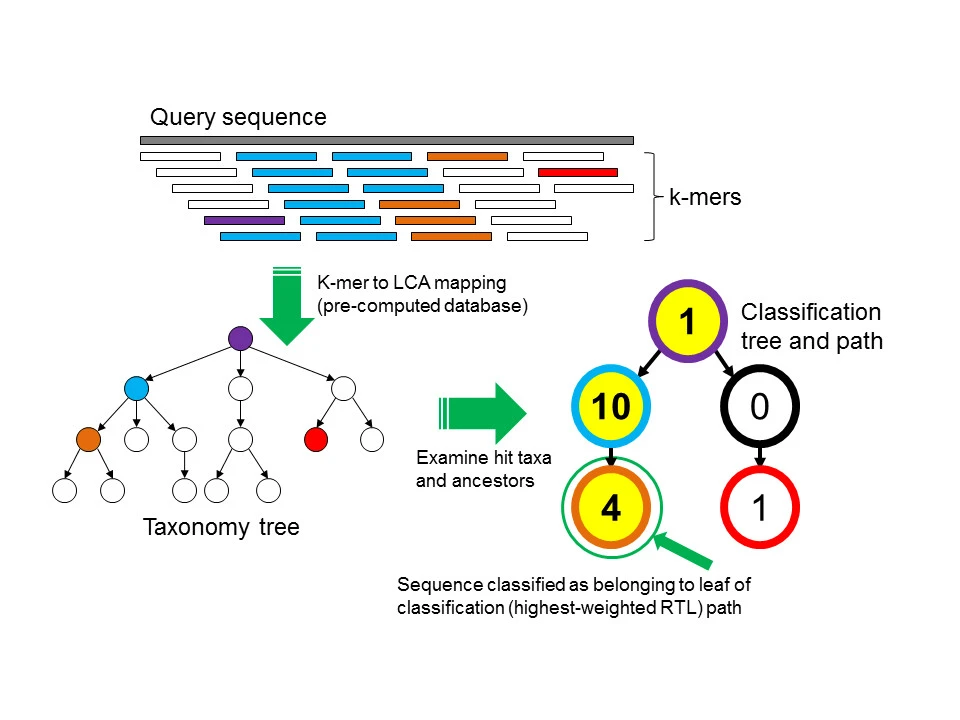
\includegraphics[scale=0.3]{Img/cap1/kraken.png}
%\caption{kraken}
%\end{figure}

BRACKEN (Bayesian Re-estimation of Abundance after Classification with KraKEN) calcula la abundancia de especies, géneros u otras categorías taxonómicas a partir de las secuencias de ADN recopiladas en un experimento de metagenómica (Lu et al., 2017)(\cite{lu2017bracken}).\\

BRACKEN realiza estimaciones probabilísticas basadas en las salidas de Kraken para completar las asignaciones al nivel taxonómico requerido, con el objetivo de obtener una estimación de abundancia más precisa. Este enfoque permite producir estimaciones fiables de abundancia a nivel de especie y género, incluso cuando una muestra contiene múltiples especies casi idénticas.\\

\section{Lenguajes}

\subsection{BASH}
Bash (Bourne Again SHell) es un intérprete de comandos y un lenguaje de scripting desarrollado para el sistema operativo Unix y sus derivados, como Linux. Creado en 1989 por Brian Fox, Bash permite automatizar tareas mediante scripts, lo que resulta particularmente útil en entornos de análisis bioinformático, donde se requiere manejar grandes volúmenes de datos. Aunque no está diseñado específicamente para análisis estadísticos o gráficos, Bash es fundamental para la gestión de flujos de trabajo y la integración de herramientas como BLAST, SAMtools y GATK. Se emplea para procesar datos en sistemas de alto rendimiento, administrar flujos de trabajo de análisis masivo y realizar manipulaciones rápidas de datos en formatos de texto o binarios. \\

\subsection{Python}
Python es un lenguaje de programación de propósito general, conocido por su sintaxis sencilla y su amplia aplicabilidad en la ciencia de datos, bioinformática y aprendizaje automático. Fue creado por Guido van Rossum en 1991 y se ha consolidado como una herramienta versátil en disciplinas científicas debido a su capacidad para integrar múltiples flujos de trabajo. Python cuenta con bibliotecas científicas robustas, como NumPy para álgebra lineal, Pandas para manejo de datos estructurados y Biopython para análisis bioinformáticos. Se emplea en la automatización de procesos, el desarrollo de algoritmos personalizados, el análisis de secuencias genómicas y la inteligencia artificial aplicada a la investigación científica.\\

\subsubsection{Phyloseq}
Phyloseq es un software de código abierto diseñado para la manipulación y análisis integral de datos metagenómicos generados mediante tecnologías de secuenciación de alto rendimiento. Esta herramienta, desarrollada en R, ofrece capacidades para importar, almacenar, analizar y visualizar datos metagenómicos de manera eficiente. En el entorno de R, los datos se estructuran en un objeto Phyloseq, que tiene la versatilidad de contener elementos clave, como la tabla de taxonomía, la tabla de conteos, la tabla de muestras o metadatos, y el árbol filogenético. Esta organización multifacética facilita un análisis completo y preciso de la estructura de la comunidad microbiana, brindando una comprensión profunda de los datos metagenómicos. (\cite{mcmurdie2013})\\

\begin{figure}[h]
\centering
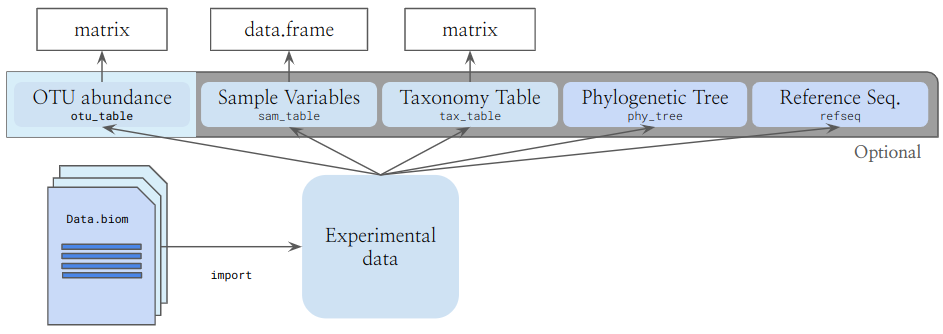
\includegraphics[width=\textwidth]{Img/cap2/Phyloseq.png}
\caption{Objeto phyloseq }%\citep{Introducción a phyloseq-castrolab})}
\end{figure}

\subsection{R \& RStudio}
R es un lenguaje de programación y un entorno de software diseñado específicamente para el análisis estadístico y la visualización de datos. Desarrollado inicialmente por Ross Ihaka y Robert Gentleman en 1993, se ha convertido en una herramienta esencial en biología, ecología, genómica y otras disciplinas científicas que requieren análisis cuantitativos. Su principal fortaleza radica en la disponibilidad de bibliotecas especializadas, como ggplot2 para visualización y phyloseq para análisis de microbiomas, además de su comunidad activa, que contribuye con paquetes de código abierto. R se utiliza ampliamente en análisis de datos complejos, modelado estadístico, aprendizaje automático y visualización avanzada, facilitando la reproducibilidad y el manejo de grandes volúmenes de datos.\\

RStudio es un entorno de desarrollo integrado (IDE) diseñado para trabajar con el lenguaje de programación R. Ofrece una interfaz intuitiva que facilita la escritura, ejecución y depuración de código, así como la visualización de resultados. RStudio permite organizar proyectos, gestionar paquetes y bibliotecas, y crear documentos reproducibles con R Markdown. También es compatible con Shiny para aplicaciones interactivas. Disponible en versiones gratuitas y de pago, RStudio es ideal tanto para principiantes como para expertos en análisis de datos.\\

\section{Formatos}

\subsection{JSON}
JSON (JavaScript Object Notation) es un formato de texto ligero para el intercambio de datos estructurados, representado como pares clave-valor u objetos anidados. En bioinformática, se utiliza comúnmente para almacenar metadatos y resultados jerarquizados debido a su compatibilidad con múltiples lenguajes de programación y su facilidad de lectura. Se emplea frecuentemente para guardar información de taxonomía, anotaciones funcionales o resultados de herramientas como QIIME 2, que lo usa para almacenar objetos complejos, como árboles filogenéticos y tablas de abundancia.\\

\subsection{BIOM}
El formato BIOM (Biological Observation Matrix) es un estándar binario utilizado en bioinformática para almacenar matrices de datos biológicos, especialmente en estudios de microbiomas. Facilita el almacenamiento eficiente de datos de abundancia y metadatos asociados, y es compatible con herramientas como QIIME y Phyloseq. El formato contiene tablas de abundancia con taxones como filas, muestras como columnas y valores numéricos que representan abundancias relativas o absolutas. Además, permite incluir metadatos sobre muestras y taxones, como información ambiental o taxonómica.\\

\subsection{FASTA}
FASTA (Fast Alignment Search Tool-All) es un formato de texto plano que almacena secuencias de ADN, ARN o proteínas. Cada entrada contiene un encabezado (precedido por "\>") seguido de una línea con la secuencia biológica. Es ampliamente utilizado para compartir datos genómicos y transcriptómicos.\\

FASTQ es un formato que extiende FASTA, añadiendo información sobre la calidad de cada nucleótido o aminoácido. Es fundamental para los datos generados por plataformas de secuenciación de próxima generación (NGS). Cada entrada en FASTQ tiene cuatro líneas:
\begin{enumerate}
\item Un identificador de la secuencia.
\item La secuencia biológica.
\item Un separador "$+$".
\item Una línea con la puntuación de calidad (en formato ASCII).
\end{enumerate}

\subsection{BAM}
BAM (Binary Alignment/Map) es un formato binario utilizado para almacenar datos de alineamiento de secuencias genómicas. Es una versión comprimida y binaria del formato SAM (Sequence Alignment/Map), que es un formato de texto para almacenar los mismos datos. BAM es ampliamente utilizado en bioinformática, especialmente en análisis de datos de secuenciación de próxima generación (NGS), debido a su eficiencia en el almacenamiento y procesamiento de grandes volúmenes de datos.\\

Cada archivo BAM contiene información detallada sobre cómo las secuencias de ADN se alinean con una referencia genómica, incluyendo la posición de la secuencia en el genoma, la calidad del alineamiento, las secuencias de los nucleótidos y las puntuaciones de calidad. Dado que el formato BAM es binario, es más compacto y rápido de manejar en comparación con su contraparte en texto, SAM.\\

\section{Solena}
Solena es una empresa de biotecnología agrícola (AgTech) enfocada en el análisis y mejora del microbioma del suelo. Su misión es desarrollar soluciones innovadoras basadas en datos moleculares y biotecnología para optimizar la salud del suelo y, como consecuencia, aumentar la productividad agrícola. Aprovechando herramientas avanzadas como inteligencia artificial y genómica, Solena obtiene conocimientos profundos sobre la composición y funcionalidad del microbioma del suelo. Además, en colaboración con organizaciones locales, la empresa implementa centros de diagnóstico molecular agrícola, como el establecido en México, para evaluar la salud de los suelos y fomentar prácticas agrícolas regenerativas.



\section{fresa}

rizosfera 
datos de fresas 
plantas sanasy enfermas 
El estudio investiga las diferencias en la estructura y diversidad de la comunidad microbiana del suelo rizosférico asociadas a plantas de fresa (Fragaria × ananassa) infectadas y no infectadas con el oídio (Podosphaera aphanis). Utilizando tecnología de secuenciación de alto rendimiento (Illumina MiSeq), se analizaron las comunidades microbianas para evaluar los efectos del patógeno sobre la microbiota del suelo en condiciones controladas de invernadero. El objetivo principal fue caracterizar las diferencias en la composición y diversidad microbiana de la rizosfera entre plantas infectadas y no infectadas, explorando posibles relaciones entre la infección por oídio y cambios en el microbioma rizosférico.(yang2020comparison)\\


\section{Simuladores de Secuencias metagenomicas}

CAMISIM es un simulador de secuencias metagenómicas, este software puede simular una amplia variedad de comunidades microbianas y conjuntos de datos metagenomicos, este algoritmo se divide en tres partes, la primera es el diseño de la comunidad, aqui se crean dichos datos a partir de perfiles taxonomicos de novo o de una base de datos genomicos dada (\cite{fritz2019camisim}). Para el diseño a partir de perfiles taxonomicos, se incluye una base de datos de la taxonomia de NCBI (National Center for Biotechnology Information), y se proporcionan en formato BIOM (Biological Observation Matrix format); estos perfiles pueden incluir taxones de bacterias,arqueas y eucariotas asi como virus. Para el diseño de comunidad de novo, se necesitan genomas en formato .fasta y un archivo de mapeo que contenga ID taxonomico (de NCBI) y OTU para cada genoma.  \\

En segunda parte se basa en la simulacion del metagenoma, los conjuntos de datos del metagenoma se generan a partir de los perfiles de abundancia y genomas del paso anterior; las longitudes de los reads y los tamaños de los insertos se pueden variar para algunos simuladores. Para cada conjunto de datos, CAMISIM genera archivos FASTQ y un archivo BAM.  \\

Y por ultimo en la tercera parte se tiene la creación y posprocesamiento de estandares de oro de ensamblaje y agrupacion, a partir de los datos del metagenoma simulado,los archivos FASTQ y BAM. CAMISIM genera los estándares de oro del genoma y el taxón para las lecturas y los contigs ensamblados, respectivamente. Estos especifican el genoma y el linaje taxonómico al que pertenecen las secuencias individuales. Todas las secuencias se pueden anonimizar y mezclar (pero rastrear durante todo el proceso), para permitir su uso en desafíos de evaluación comparativa.  \\

\begin{itemize}
    \item CAMISIM es un programa flexible para simular una gran variedad de comunidades microbianas y muestras de metagenomas. 
    \item Posee un conjunto de funciones completo para simular comunidades microbianas realistas y conjuntos de datos de metagenomas.
    \item Exploraron el efecto de las propiedades específicas de los datos en el rendimiento del ensamblador.
\end{itemize}



DeepMAsED tiene un enfoque de deeplearning para identificar contig  mal ensamblados sin necesidad de genomas de referencia.\\



